\documentclass[a4paper,11pt]{article}
\usepackage{amsmath,amsthm,amsfonts,amssymb,amscd,amstext,vmargin,graphics,graphicx,tabularx,multicol} 
\usepackage[francais]{babel}
\usepackage[utf8]{inputenc}  
\usepackage[T1]{fontenc} 
\usepackage{pstricks-add,tikz,tkz-tab,variations}
\usepackage[autolanguage,np]{numprint} 
\usepackage{calc}
\usepackage{mathrsfs}

\usepackage{cancel}

\setmarginsrb{1.5cm}{0.5cm}{1cm}{0.5cm}{0cm}{0cm}{0cm}{0cm} %Gauche, haut, droite, haut
\newcounter{numexo}
\newcommand{\exo}[1]{\stepcounter{numexo}\noindent{\bf Exercice~\thenumexo} : }
\reversemarginpar

\newcommand{\bmul}[1]{\begin{multicols}{#1}}
\newcommand{\emul}{\end{multicols}}

\newcounter{enumtabi}
\newcounter{enumtaba}
\newcommand{\q}{\stepcounter{enumtabi} \theenumtabi.  }
\newcommand{\qa}{\stepcounter{enumtaba} (\alph{enumtaba}) }
\newcommand{\initq}{\setcounter{enumtabi}{0}}
\newcommand{\initqa}{\setcounter{enumtaba}{0}}

\newcommand{\be}{\begin{enumerate}}
\newcommand{\ee}{\end{enumerate}}
\newcommand{\bi}{\begin{itemize}}
\newcommand{\ei}{\end{itemize}}
\newcommand{\bp}{\begin{pspicture*}}
\newcommand{\ep}{\end{pspicture*}}
\newcommand{\bt}{\begin{tabular}}
\newcommand{\et}{\end{tabular}}
\renewcommand{\tabularxcolumn}[1]{>{\centering}m{#1}} %(colonne m{} centrée, au lieu de p par défault) 
\newcommand{\tnl}{\tabularnewline}

\newcommand{\trait}{\noindent \rule{\linewidth}{0.2mm}}
\newcommand{\hs}[1]{\hspace{#1}}
\newcommand{\vs}[1]{\vspace{#1}}

\newcommand{\N}{\mathbb{N}}
\newcommand{\Z}{\mathbb{Z}}
\newcommand{\R}{\mathbb{R}}
\newcommand{\C}{\mathbb{C}}
\newcommand{\Dcal}{\mathcal{D}}
\newcommand{\Ccal}{\mathcal{C}}
\newcommand{\mc}{\mathcal}

\newcommand{\vect}[1]{\overrightarrow{#1}}
\newcommand{\ds}{\displaystyle}
\newcommand{\eq}{\quad \Leftrightarrow \quad}
\newcommand{\vecti}{\vec{\imath}}
\newcommand{\vectj}{\vec{\jmath}}
\newcommand{\Oij}{(O;\vec{\imath}, \vec{\jmath})}
\newcommand{\OIJ}{(O;I,J)}


\newcommand{\reponse}[1][1]{%
\multido{}{#1}{\makebox[\linewidth]{\rule[0pt]{0pt}{20pt}\dotfill}
}}

\newcommand{\titre}[5] 
% #1: titre #2: haut gauche #3: bas gauche #4: haut droite #5: bas droite
{
\noindent #2 \hfill #4 \\
#3 \hfill #5

\vspace{-1.6cm}

\begin{center}\rule{6cm}{0.5mm}\end{center}
\vspace{0.2cm}
\begin{center}{\large{\textbf{#1}}}\end{center}
\begin{center}\rule{6cm}{0.5mm}\end{center}
}



\begin{document}
\pagestyle{empty}
\titre{Séance d'exercices: Résolution d'équation du premier degré}{}{}{3ème}{}

\vspace*{0.2cm}


{\large \textbf{\underline{PARTIE A :}}  Résolution d'équation}\\

\vspace*{0.25cm}

\exo \\


\initq \textbf{\qa} On considère l'équation suivante : \hspace*{0.5cm} $ 5x + 3(8-2x) = 15-(x-9)$\\
\textbf{4 est-il solution de l'équation ?}\\

\color{red}
\bmul{2}
D'une part, $ 5 \times 4 + 3 \times (8 - 2 \times 4)  = 20 + 3 \times (8-8)$\\

 \hspace*{5.65cm}$= 20 + 0$\\

 \hspace*{5.55cm} $=\underline{20}$\\

\columnbreak

D'autre part, $15 -(4-9) = 15 -(-5) $\\

 \hspace*{4.5cm}$=15 + 5$\\

\hspace*{4.5cm} $= \underline{20}$
\emul

L'égalité est donc  vérifiée pour $x=4$.\\
\color{black}

\qa On considère l'équation suivante : \hspace*{0.5cm} $(3x+2)^{2} = 9x^{2} + 6x + 4$\\
\textbf{-2 est-il solution de l'équation ?}\\

\color{red}
\bmul{2}
D'une part, $ (3 \times (-2)+2)^{2} = (-6 + 2 )^{2}$\\

 \hspace*{4.75cm}$= (-4)^{2}$\\

 \hspace*{4.65cm} $=\underline{16}$\\

\columnbreak

D'autre part, $9 \times (-2)^{2} + 6 \times (-2) +4 = 9 \times 4 -12 +4 $\\

 \hspace*{6.25cm}$=36-12+4$\\

\hspace*{6.05cm} $= \underline{28}$
\emul

L'égalité n'est donc pas vérifiée pour $x=4$.\\
\color{black}

\vspace{0.5cm}

\exo 

Résoudre les équations suivantes.


\bmul{3}
\initqa 

\qa $$-2+x=11$$

\color{red}
$$-2 + x + 2 = 11 + 2$$

$$\fbox{x = 13}$$

\color{black} 

\qa $$\dfrac{3}{4}x=5$$

\color{red}

$$ \dfrac{\dfrac{3}{4}x}{\dfrac{3}{4}}= \dfrac{5}{\dfrac{3}{4}}$$

$$x= 5 \times \dfrac{4}{3}$$

$$x = \dfrac{20}{3} $$

\color{black} 

\columnbreak

\qa $$9+x=44$$


\color{red}

$$9+x-9 = 44-9$$

$$\fbox{x =35}$$
\color{black} 

\qa $3x=27$\\

\color{red}

$$ \dfrac{3x}{3}= \dfrac{27}{3}$$



$$\fbox{x =9}$$

\color{black} 


\columnbreak

\qa $$-6 +x =-41$$


\color{red}

$$-6 + x + 6 =-41 +6$$


$$\fbox{x =-35}$$

\color{black} 

\qa $-6x=-42$\\

\color{red}

$$ \dfrac{-6x}{-6}= \dfrac{-42}{-6}$$



$$\fbox{x =7}$$

\color{black} 

\emul

\newpage
\exo 

Résoudre les équations suivantes.


\bmul{3}
\initqa 

\textbf{a)} $$ 4x - 3 = 79$$
\color{red}
$$ 4x -3 +3 = 79 +3 $$

$$ 4x  =  82$$

$$ \dfrac{4x}{4}  =  \dfrac{82}{4}$$

$$\fbox{x =20,5}$$
\color{black}

\textbf{b)} $$4x-7 = 3x+8$$

\color{red}
$$ 4x -7-3x = 3x+8 -3x$$

$$x-7  =  8$$

$$x-7+ 7 =  8+7$$

$$\fbox{x =15}$$
\color{black}






\columnbreak

\textbf{d)} $$6-8x=16x$$

\color{red}
$$ 6-8x-16x= 16x-16x $$

$$ 6-24x  =  0$$

$$ 6-24x -6 =  0-6$$

$$ -24x  =  -6$$

$$ \dfrac{-24x}{-24}  =  \dfrac{-6}{-24}$$

$$x = \dfrac{1}{4}$$

\color{black}


\textbf{e)} $$-x+11 = \dfrac{3}{5} x+3$$

\color{red}
$$ -x+11-\dfrac{3}{5}x = \dfrac{3}{5} x+3 - \dfrac{3}{5}x $$

$$ \dfrac{-5}{5}x -\dfrac{3}{5}x +11  =  3$$

$$ \dfrac{-8}{5}x  +11  =  3$$

$$ \dfrac{-8}{5}x  +11 -11 =  3-11$$

$$ \dfrac{-8}{5}x   =  -8$$

$$ \dfrac{-\dfrac{8}{5}x }{-\dfrac{8}{5}} =  \dfrac{-8}{\dfrac{-8}{5}}$$

$$ x =  -8  \times  \dfrac{-5}{8}$$



$$\fbox{x =5}$$
\color{black}





\columnbreak

\textbf{g)} $50 = -2x + 35$


\color{red}
$$ 50-35= -2x +35 -35$$

$$15  =  -2x$$


$$ \dfrac{15}{-2}  =  \dfrac{-2x}{-2}$$

$$\fbox{-7,5 = x}$$

$$\fbox{x = -7,5}$$

\color{black}


\textbf{h)} $$-2x +5 = -8x + 10$$

\color{red}
$$-2x+5+8x= -8x+10+8x $$

$$ 6x +5 =  10$$

$$6x+5-5= 10-5$$

$$ 6x =  5$$

$$ \dfrac{6x}{6}  =  \dfrac{5}{6}$$

$$x = \dfrac{5}{6}$$

\color{black}


\emul

\newpage




\bmul{3}

\textbf{c)} $$ 3 -(5x+1) = 8x +(4-2x)$$

\color{red}
$$3-5x-1= 8x+4-2x $$

$$2-5x= 6x+4 $$

$$ 2-5x-6x =  6x+4-6x$$

$$2-11x= 4$$

$$2-11x -2= 4-2$$

$$ -11x = 2$$

$$ \dfrac{-11x}{-11}  =  \dfrac{2}{-11}$$

$$x = -\dfrac{2}{11}$$

\color{black}

\columnbreak

\textbf{f)} $$7(2x+5) - 3x = 5 + 8x $$

\color{red}
$$ 14x +35 -3x= 5+8x$$

$$11x+35-8x= 5+8x-8x$$

$$3x+35= 5$$

$$3x+35-35= 5-35$$

$$3x = -30$$

$$\dfrac{3x}{3}= \dfrac{-30}{3}$$

$$\fbox{x =-10}$$
\color{black}

\columnbreak


\textbf{i)} $$( x - 1)( x + 3) = ( x + 5)( x - 4) $$
\color{red}
 $$x^{2} +3x-x-3 = x^{2}-4x+5x-20 $$

 $$x^{2} +2x-3 = x^{2}+x-20 $$
 
  $$x^{2} +2x-3 -x^{2} = x^{2}+x-20 -x^{2}$$
  
   $$ 2x-3 = x-20 $$
   
    $$ 2x-3-x = x-20-x $$
    
     $$ x-3 =-20 $$
   
 $$ x-3+3 =-20+3$$
 
 
$$\fbox{x =-17}$$
 

\color{black}
\emul

{\large \textbf{\underline{PARTIE B :}} Mise en équation} \\

\vspace*{0.5cm}


 
 
 
 \exo
 
 Trouve un nombre sachant que son triple augmenté de 2 est égal à son double augmenté de 3.\\
 
 \color{red}
On appelle $x$ le nombre recherché.\\


L'équation est la suivante : \hspace*{1cm} $3x+2=2x+3$ 

$$3x+2-2x=2x+3-2x$$

$$x+2=3$$

$$x+2-2=3-2$$
 
 $$x=1$$
 
 Le nombre recherché est 1.\\
 
 \textbf{Vérification :} $ 3 \times 1 + 2 = 5$ et $2 \times 1 + 3 = 5$ \\
 
 \color{black}


\vspace*{0.5cm}

\exo\\

Noah veut acheter des livres qui coûtent le même prix.\\
S'il en achète 7, il lui manque 1,20 euros. S'il en achète 6, il lui reste 3,50 euros.\\

Quel est le prix d'un livre ?\\


\color{red}
On appelle $x$ le prix d'un livre.\\

L'équation est la suivante : \hspace*{1cm} $7x-1,20= 6x+3,50$ 


$$7x-1,20-6x= 6x+3,50-6x$$

$$x-1,20= 3,50$$

$$x-1,20+1,20=3,50+1,20$$

$$x=4,70$$

Un livre coûte 4,70 euros.\\

 \color{black}
\vspace*{0.5cm}

\exo \\

Deux frères, Marc et Jean, possèdent chacun un jardin. L'aire du jardin de Marc vaut les $\dfrac{3}{4}$ de l'aire du jardin de Jean. Les deux frères possèdent en tout 1 470 $ m^{2} $.\\

Quelles sont les aires des jardins de Marc et de Jean  ?\\

\color{red}


On appelle $x$, l'aire du terrain de Jean.\\

Pour trouver l'équation, il faut choisir une grandeur qui peut être exprimée de deux façons différentes.\\

Ici, il s'agit de l'aire du jardin qu'ils ont à eux 2.\hspace*{1cm} \textbf{Il y a 1 470 $m^{2}$ en tout}.\\

Mais cela peut aussi s'écrire : \textbf{Aire de Jean + Aire de Marc.}\\

On sait que :
\bi
\item \textcolor{green}{Aire de Jean = x}

\item l'aire du jardin de Marc vaut les $\dfrac{3}{4}$ de l'aire du jardin de Jean. , à savoir \textcolor{blue}{Aire de Marc = $\dfrac{3}{4}x$ }

\ei

L'équation est donc la suivante : \hspace*{1cm} $ \textcolor{green}{Aire de Jean } + \textcolor{blue}{Aire de Marc}  = 1 470$\\

$$ x + \dfrac{3}{4}x = 1470$$


$$ \dfrac{4}{4}x + \dfrac{3}{4}x = 1470$$

$$ \dfrac{7}{4}x = 1470$$

$$ \dfrac{\dfrac{7}{4}x}{\dfrac{7}{4}} = \dfrac{1470}{\dfrac{7}{4}}$$


$$x = \dfrac{1470}{\dfrac{7}{4}}$$


$$x =1470 \times \dfrac{4}{7}$$

$$x =840$$

Donc, l'aire du terrain de Jean vaut 840 $m^{2}$.\\

Pour Marc : $\dfrac{3}{4} \times 840 = 630 m^{2}$ \hspace*{1.5cm}\textbf{Vérification :} 840 + 630 = 1 470.\\



\color{black}


 \newpage
 
 \exo

Thomas a obtenu 11 et 16 aux deux premiers contrôles de Maths.\\
Quelle note doit-il avoir au troisième contrôle pour obtenir 15 de moyenne ?\\

\color{red}
On appelle $x$ la troisième note.\\

$$\dfrac{11 + 16 + x}{3}=15$$

$$\dfrac{27 + x}{3}=15$$

$$\dfrac{(27+ x)\times \cancel{3}}{\cancel{3}}=15 \times 3$$


$$27+ x=15 \times 3$$

$$27+ x=45$$

$$27+ x-27=45-27$$

$$ \fbox{ x=18}$$

La troisième note de Thomas doit être un 18 pour obtenir 15 de moyenne.\\

\color{black}

 
 
\exo\\
 \textbf{Trouver la valeur de x pour que l'aire de AMNP soit égale au tiers de l'aire du carré ABCD.}\\
 Justifier votre réponse à l'aide d'une équation.\\


\begin{center}
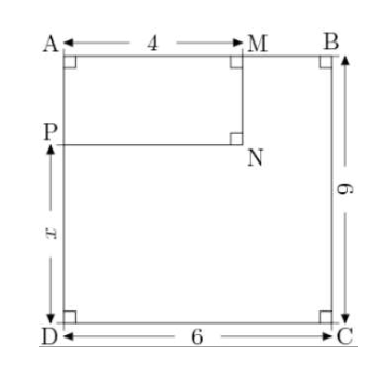
\includegraphics[scale=0.9]{carre.eps} 

\end{center}

\textit{\underline{Indication : } Exprimer l'aire du rectangle AMNP en fonction de x et l'aire du carré ABCD.}\\ 

\color{red}
On appelle $x$ la longueur DP.\\


Dans l'énoncé, il est question de l'aire du rectangle AMNP et de l'aire du carré ABCD.\\
On va donc essayer de les exprimer  :\\

- $A_{ABCD} = 6 \times 6$ \hspace*{1cm} $A_{ABCD} = 6 \times 6 = \underline{36} $ \\

- $A_{AMNP} = L \times l = \underline{4 \times (6-x)}$\\

On trouve donc l'équation suivante : \hspace*{1cm} $A_{AMNP} = \dfrac{A_{ABCD}}{3}$\\

$$4(6-x)=\dfrac{36}{3} $$

$$24-4x=12 $$

$$24-4x -24=12-24 $$

$$-4x = -12 $$

$$\dfrac{-4x}{-4}= \dfrac{-12}{-4} $$

$$ \fbox{x = 3} $$


On trouve donc que pour x = 3, l'aire de AMNP soit égale au tiers de l'aire du carré ABCD.\\


\textbf{Vérification :} \\
- $A_{ABCD} = 6 \times 6 = 36$ \\

- $A_{AMNP} = L \times l = 4 \times 3 = 12$\\

et $36 \div 3 = 12$\\

\color{black}
\vspace*{0.5cm}

\exo\\


Le point M se déplace sur le segment [AC]. \\
Est-il possible que les rectangles ADM et EMC aient la même aire ? Justifier votre réponse à l'aide d'une résolution d'équation.\\



\begin{center}
\includegraphics[scale=0.7]{equation.eps} 

\end{center}

\textit{\underline{Indication : } Exprimer l'aire des deux triangles en fonction de x.}\\ 



\end{document}
